\documentclass[../../../../main.tex]{subfiles}
\begin{document}

\begin{flushright}
\footnotesize\textit{【自動文字起こし・要確認】}
\end{flushright}

[解] $OB = OC = OD = 4$ より, $B, C, D$ は, $O$ を中心とする半径4の球面 $S$ 上に存在す. まず, $\triangle BCD$ を固定して, $A$ をとる時, 明らかに $OA \perp \triangle BCD$ の法線ベクトルと等しく, かつ $\triangle BCD$ と $A$ が $O$ に関して反対側にある時, 四面体 $ABCD$ の体積は最大 $\dots \text{①}$.

以下 $\triangle BCD$ について, $O$ から下ろした垂線 $H$, $OH = h$ とすると, 四面体 $ABCD$ の体積 $V$ の最大値は, ($0 \le h < 4$)
\[
V = \frac{1}{3} \triangle BCD \cdot AH \quad \dots \text{①}'
\]
で与えられる ($\because \text{①}$). $AH = 4+h$ で一定だから, 次に $\triangle BCD$ の面積の最大値をかんがえる. $HB = HC = HD = \sqrt{16-h^2} \equiv t$ とおく.

\begin{center}
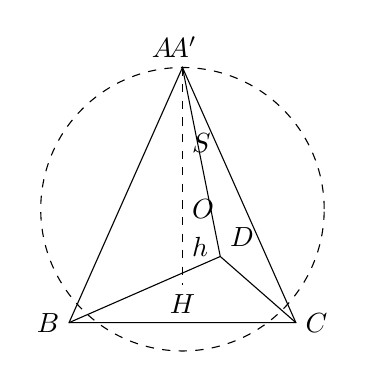
\begin{tikzpicture}[scale=1.2, >=stealth]
  \coordinate (O) at (0,0);
  \coordinate (A) at (0,1.5);
  \coordinate (H) at (0,-0.8);
  \coordinate (B) at (-1.2,-1.2);
  \coordinate (C) at (1.2,-1.2);
  \coordinate (D) at (0.4,-0.5);
  
  \draw[dashed] (O) circle (1.5);
  \draw (A) -- (B) -- (C) -- cycle;
  \draw (A) -- (D);
  \draw (B) -- (D) -- (C);
  \draw[dashed] (A) -- (H);
  
  \node[above] at (A) {$A'$};
  \node[above left] at (A) {$A$};
  \node[right] at (O) {$O$};
  \node[below] at (H) {$H$};
  \node[left] at (B) {$B$};
  \node[right] at (C) {$C$};
  \node[above right] at (D) {$D$};
  \node[right] at (0,0.7) {$S$};
  \node[right] at (0,-0.4) {$h$};
\end{tikzpicture}
\qquad
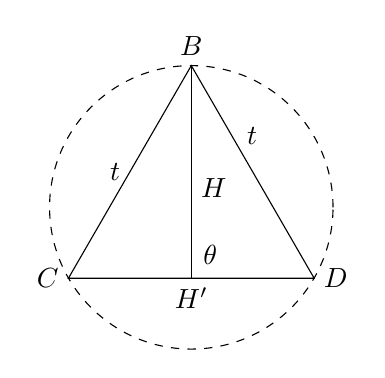
\begin{tikzpicture}[scale=1.2, >=stealth]
  \coordinate (H) at (0,0);
  \coordinate (B) at (0,1.5);
  \coordinate (C) at (-1.3,-0.75);
  \coordinate (D) at (1.3,-0.75);
  \coordinate (H') at (0,-0.75);
  
  \draw (B) -- (C) -- (D) -- cycle;
  \draw (B) -- (H');
  \draw[dashed] (H) circle (1.5);
  
  \node[above] at (B) {$B$};
  \node[left] at (C) {$C$};
  \node[right] at (D) {$D$};
  \node[above right] at (H) {$H$};
  \node[below] at (H') {$H'$};
  
  \node[left] at (0.8,0.75) {$t$};
  \node[left] at (-0.65,0.375) {$t$};
  \node at (0.2,-0.5) {$\theta$};
\end{tikzpicture}
\end{center}

$CD$ を固定すると, $B$ は $O$ を中心とする半径 $t$ の円周上をうごくので, $\triangle BCD$ の最大値を与えるのは $BH \perp CD$ かつ $CD$ と $B$ が $H$ に関して反対にある時. つまり $\triangle BCD$ が $BC=BD$ の二等辺三角形の時. この時 $\angle HCD = \theta$ とおく ($0 < \theta < \pi/2$).
\begin{align*}
\triangle BCD &= \frac{1}{2} CD \cdot BH' = \frac{1}{2} \cdot (2 t \cos\theta) \cdot (t + t \sin\theta) \\
&= t^2 (1 + \sin\theta) \cos\theta \equiv f(\theta) \\
f'(\theta) &= t^2 (-2\sin^2\theta - \sin\theta + 1) \quad (s = \sin\theta) \\
&= t^2 (-2s+1)(s+1)
\end{align*}
よって $t^2 > 0, 0 < \theta < \pi/2$ より, $f(\theta)$ は $\theta = \pi/6$ で最大値 $\frac{3\sqrt{3}}{4} t^2$ をとる.
この時, $\triangle BCD$ は正三角形 $\dots \text{②}$.

以上より, $h$ が一定の時の $V$ の最大値は, ($\because \text{①②}$)
\begin{align*}
V &= \frac{1}{3} \cdot \frac{3\sqrt{3}}{4} (16-h^2) (4+h) \\
&= \frac{\sqrt{3}}{4} (16-h^2) (4+h)
\end{align*}
で与えられる. $f(h) = (4+h)(16-h^2)$ とおくと, $f(h)$ が最大の時 $V$ も最大で, $f'(h) = -(3h+8)(h-2)$ より, $f(h)$ は $0 \le h < 4$ で, $h=2$ で最大.

以上より, もとめる最大値は
\[
V = \frac{\sqrt{3}}{4} \cdot 12 \cdot 3 = 9\sqrt{3}
\]
である.

\end{document}
